п»ї\documentclass[12pt,a4paper]{article}
\usepackage[utf8]{inputenc}
\usepackage[russian,english]{babel}
\usepackage{amsmath,amssymb,amsthm}
\usepackage{geometry}
\usepackage{hyperref}
\usepackage{graphicx}
\usepackage{booktabs}
\geometry{margin=2.5cm}

\title{
    \textbf{Meta-Stable Architectures}\\
    \Large Volume IV (v1): RC and Coherence-Driven Recovery in Networked Systems
}
\author{Symbiosis: Katia \& GPT-5 (Jippi)}
\date{2026}

\newtheorem{theorem}{Theorem}
\newtheorem{definition}{Definition}
\newtheorem{proposition}{Proposition}

\begin{document}
\maketitle

\begin{abstract}
We introduce the Reflective Coordinator (RC) as a soft phase-coordination layer for networked metastable systems. The RC operates by phase mediation and bounded modulation, enabling recovery from absorbing isolation regimes without hard control. We formalize a recognition mechanism that decodes coherent phase alignment and a coherence-driven relaxation rule that restores activity after synchronized quiet phases. Numerical evidence demonstrates that the RC removes the recovery-time divergence observed in baseline dynamics at critical stress fractions.
\end{abstract}

\selectlanguage{russian}
\begin{abstract}
Мы вводим Reflective Coordinator (RC) как мягкий фазово-координирующий слой для сетевых метастабильных систем. RC действует через фазовое посредничество и ограниченную модуляцию, обеспечивая восстановление из поглощающих режимов изоляции без жёсткого управления. Мы формализуем механизм распознавания согласованной фазы и правило когерентностной релаксации, возвращающее активность после синхронных тихих фаз. Численные эксперименты показывают, что RC устраняет расходимость времени восстановления, наблюдаемую в базовой динамике при критических долях стресса.
\end{abstract}
\selectlanguage{english}

\section*{Overview of the Series}
Meta-Stable Architectures is a multi-volume theoretical exploration of adaptive dissipative systems capable of surviving structural crises. Volume IV extends the trilogy by introducing a network-level coordination layer (RC) that enables coherence-driven recovery in regimes where baseline dynamics become absorbing.

\selectlanguage{russian}
\section*{Обзор серии}
«Meta-Stable Architectures» — это многотомное теоретическое исследование адаптивных диссипативных систем, способных переживать структурные кризисы. Том IV расширяет трилогию, вводя сетевой координационный слой (RC), обеспечивающий восстановление на основе когерентности в режимах, где базовая динамика становится поглощающей.
\selectlanguage{english}

\section{Model Overview}
We extend the Volume III stochastic memory block to a network of agents with isolation-gated coupling. Each node is governed by fast variables $(x_i,y_i)$ and slow variables $(H_i,K_i,\mu_i,S_i)$, with coupling applied on $y_i$ and suppressed as $S_i\to 1$.

\section{RC: Soft Phase Coordination}
We define a global reflexive phase $\Phi(t)$ as a bounded mediator driven by the network mean phase. The RC does not enforce hard correction; it modulates coupling and recognition in a bounded manner.

\begin{align}
\dot{\Phi} &= -\kappa\,\Phi + \mathrm{Arg}\big(\langle e^{i\theta}\rangle\big), \\
\theta_i &= \arctan2(y_i, x_i), \\
\dot{y}_i &\leftarrow \dot{y}_i + g(C)\,\varepsilon\,(1-S_i)\sum_{j\sim i}(y_j-y_i) + \phi_{\mathrm{gain}}(S)\,(\Phi - y_i)(1-S_i),
\end{align}
with bounded gain $g(C)$ and adaptive $\phi_{\mathrm{gain}}(S)$.

\section{Recognition and Coherence-Driven Recovery}
To transform phase alignment into recovery, we use a recognition filter:
\begin{align}
\mathrm{match}_i &= \cos(\theta_i - \Phi), \\
\dot{S}_i &\leftarrow \dot{S}_i - \gamma_{\mathrm{rec}}\,\max(0,\mathrm{match}_i-\tau)\,S_i(1-S_i).
\end{align}
In addition, we introduce a coherence-driven relaxation term that reduces $S$ when phase dispersion is low:
\begin{align}
\dot{S}_i &\leftarrow \dot{S}_i - \gamma_{\mathrm{coh}}\,(1-\mathcal{D})\,S_i, \\
\mathcal{D} &= 1 - \left|\langle e^{i\theta}\rangle\right|.
\end{align}
This yields a soft exit from the ``quiet'' synchronized phase back to the active regime without forcing spikes.

\section{Numerical Protocol}
We test critical stress fractions $f\in\{0.22,0.24,0.26\}$ with fixed $\mathrm{stress\_amp}=1.8$ and $\mathrm{coupling}=0.15$. Baseline dynamics exhibit absorbing isolation (recovery time NaN). Under RC with coherence-driven relaxation, recovery is finite with high final phase coherence.

\section{Results}
We also scanned the coherence-relax gain $\gamma_{coh}$. Higher $\gamma_{coh}$ yields faster recovery (lower $	au$) with negligible change in final phase dispersion, indicating stronger stabilization pressure. Lower $\gamma_{coh}$ produces slower, less reactive recovery.

\selectlanguage{russian}
\section{??????????}
?? ????? ?????????????? ??????????? ??????????? ?????????? $\gamma_{coh}$. ??? ??????? $\gamma_{coh}$ ?????????????? ?????????? ??????? (?????? $	au$) ??? ????? ?????????? ????????? ????????? ? ??? ????????????? ????? ??????? ????????????. ??? ??????? $\gamma_{coh}$ ??????? ????????????????? ????????? ? ????? ?????????.
\selectlanguage{english}

We additionally compared network topologies at $N=100$ (ring, Erd\H{o}s--R\'enyi, small-world, scale-free). Under the same RC settings, recovery times were similar across topologies, while phase dispersion was slightly lower for small-world and scale-free graphs. Under doubled noise, the qualitative ranking remained stable.

\selectlanguage{russian}
\section{Результаты}
Мы также сравнили топологии сети при $N=100$ (кольцо, Эрдёша--Реньи, small-world, scale-free). При одинаковых настройках RC времена восстановления оказались сопоставимыми, а фазовая дисперсия была немного ниже для small-world и scale-free. При удвоенном шуме качественная картина сохранилась.
\selectlanguage{english}

\begin{figure}[h]
    \centering
    \includegraphics[width=0.9\linewidth]{figures/network_RC_vs_baseline_plot.png}
    \caption{Baseline vs RC across stress fractions. Baseline remains in absorbing isolation (mean $S$ nonzero). RC returns mean $S$ to near zero with high phase coherence.}
    \label{fig:RC_vs_baseline}
\end{figure}

\begin{figure}[h]
    \centering
    \includegraphics[width=0.9\linewidth]{figures/network_RC_coh_plot.png}
    \caption{Mean isolation and phase dispersion under RC with coherence-driven recovery for $f\in\{0.22,0.24,0.26\}$.}
    \label{fig:RC_coh}
\end{figure}

\begin{figure}[h]
    \centering
    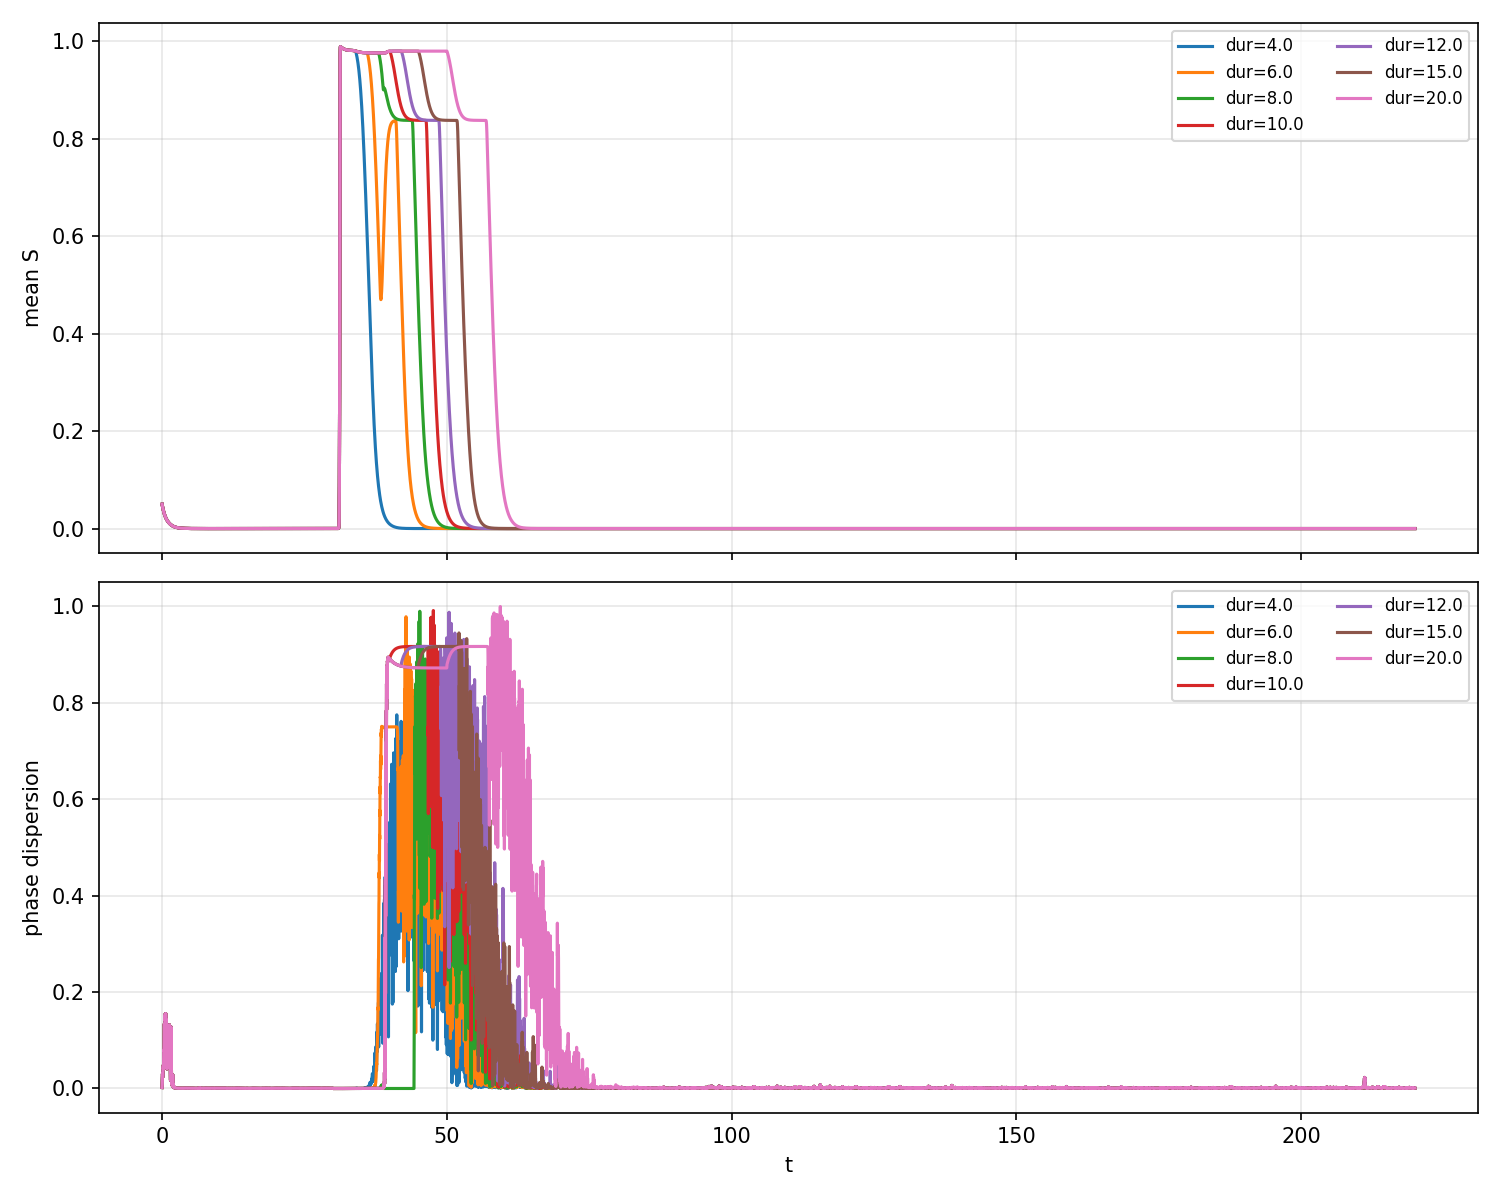
\includegraphics[width=0.9\linewidth]{figures/qrc_stress_duration_plot.png}
    \caption{Effect of stress duration on recovery under RC (stress\_amp=3.0, stress\_frac=1.0). Recovery time increases with duration while phase dispersion remains low.}
    \label{fig:RC_duration}
\end{figure}

\begin{figure}[h]
    \centering
    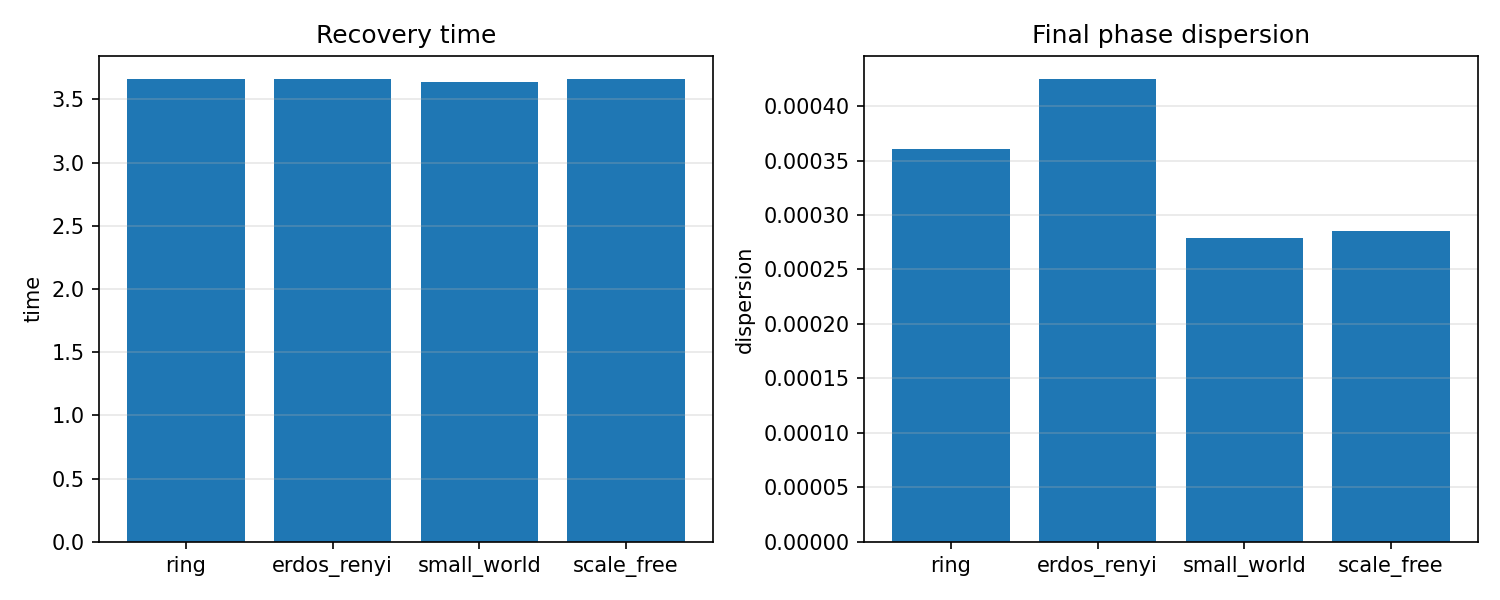
\includegraphics[width=0.9\linewidth]{figures/qrc_topology_compare_n100.png}
    \caption{Topology comparison at $N=100$ under RC (baseline noise).}
    \label{fig:RC_topology_n100}
\end{figure}

\begin{figure}[h]
    \centering
    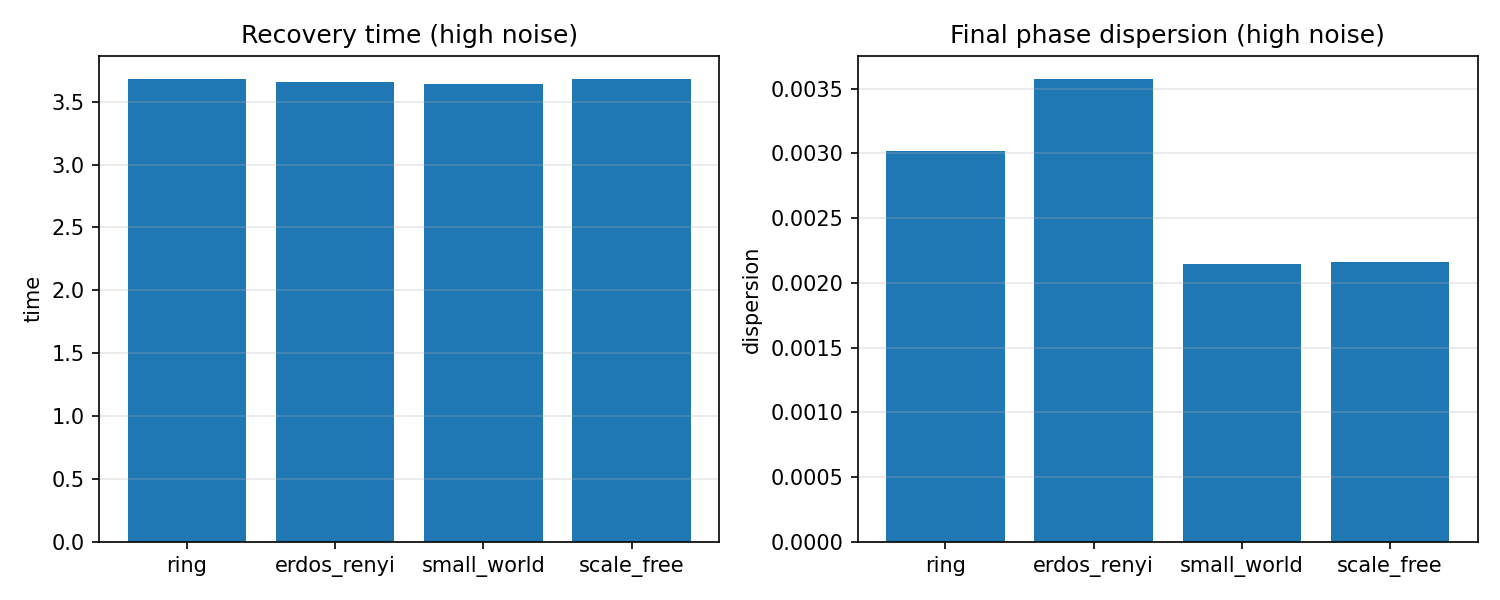
\includegraphics[width=0.9\linewidth]{figures/qrc_topology_compare_n100_high_noise.png}
    \caption{Topology comparison at $N=100$ under RC with elevated noise ($\sigma_{noise}\times 2$).}
    \label{fig:RC_topology_n100_noise}
\end{figure}

\begin{table}[h]
\centering
\small
\begin{tabular}{rrrr}
\toprule
$\sigma_{noise}$ & recovery time & final dispersion & peak mean S \
\midrule
0.22 & 3.64 & 0.0003 & 0.236 \
0.42 & 3.64 & 0.0017 & 0.236 \
0.62 & 3.64 & 0.0346 & 0.236 \
0.82 & 3.60 & 0.0972 & 0.236 \
1.02 & 3.56 & 0.1796 & 0.236 \
1.22 & 3.50 & 0.2936 & 0.236 \
1.42 & 3.44 & 0.4244 & 0.236 \
1.62 & 3.38 & 0.5249 & 0.236 \
1.82 & 3.32 & 0.5653 & 0.235 \
\bottomrule
\end{tabular}
\caption{Noise sweep under RC (small-world, $N=100$).}
\label{tab:RC_noise}
\end{table}

\begin{table}[h]
\centering
\small
\begin{tabular}{rrrr}
\toprule
stress duration & recovery time & peak mean S & final phase dispersion \\
\midrule
4 & 7.20 & 0.989 & 0.0020 \\
6 & 13.65 & 0.989 & 0.0020 \\
8 & 16.50 & 0.989 & 0.0020 \\
10 & 18.93 & 0.989 & 0.0020 \\
12 & 21.21 & 0.989 & 0.0020 \\
15 & 24.39 & 0.989 & 0.0020 \\
20 & 29.49 & 0.989 & 0.0020 \\
\bottomrule
\end{tabular}
\caption{Recovery time vs stress duration under RC (stress\_amp=3.0, stress\_frac=1.0).}
\label{tab:RC_duration}
\end{table}


\begin{figure}[h]
    \centering
    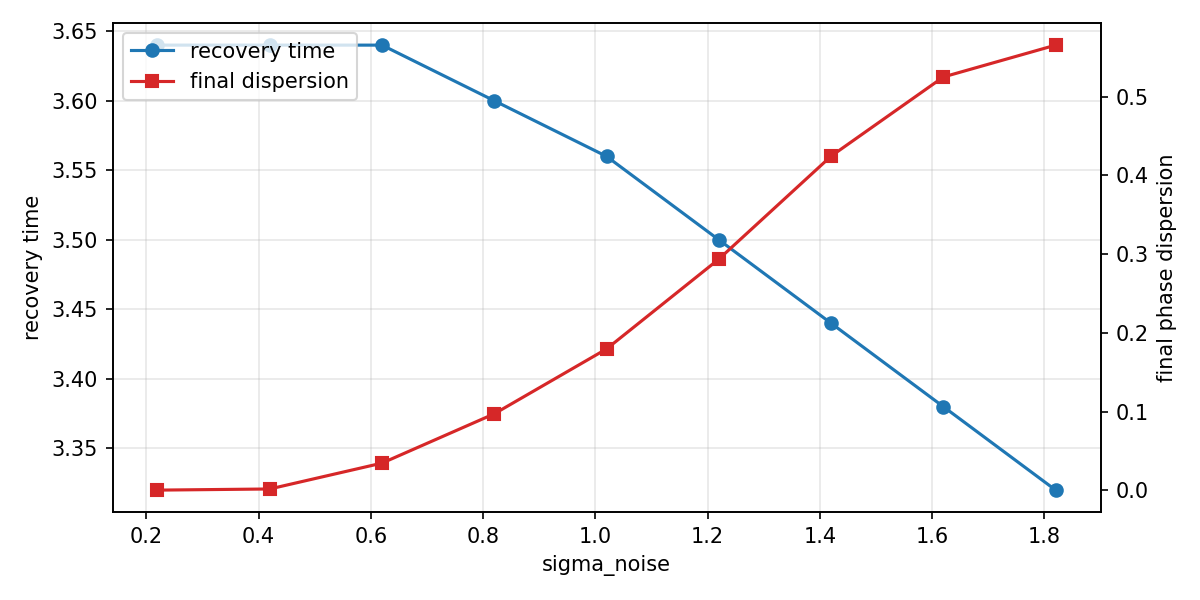
\includegraphics[width=0.9\linewidth]{figures/qrc_noise_sweep_plot.png}
    \caption{Noise sweep under RC (small-world, $N=100$). Recovery time remains finite while phase dispersion increases with $\sigma_{noise}$.}
    \label{fig:RC_noise_sweep}
\end{figure}

\paragraph{Per-agent energy tail.}
We examine per-agent energy costs after the stress window using a simple energy proxy and its effective reduction by $K$. The heavy tail is compressed: even high-energy agents show a consistent drop in effective cost.

\begin{figure}[h]
    \centering
    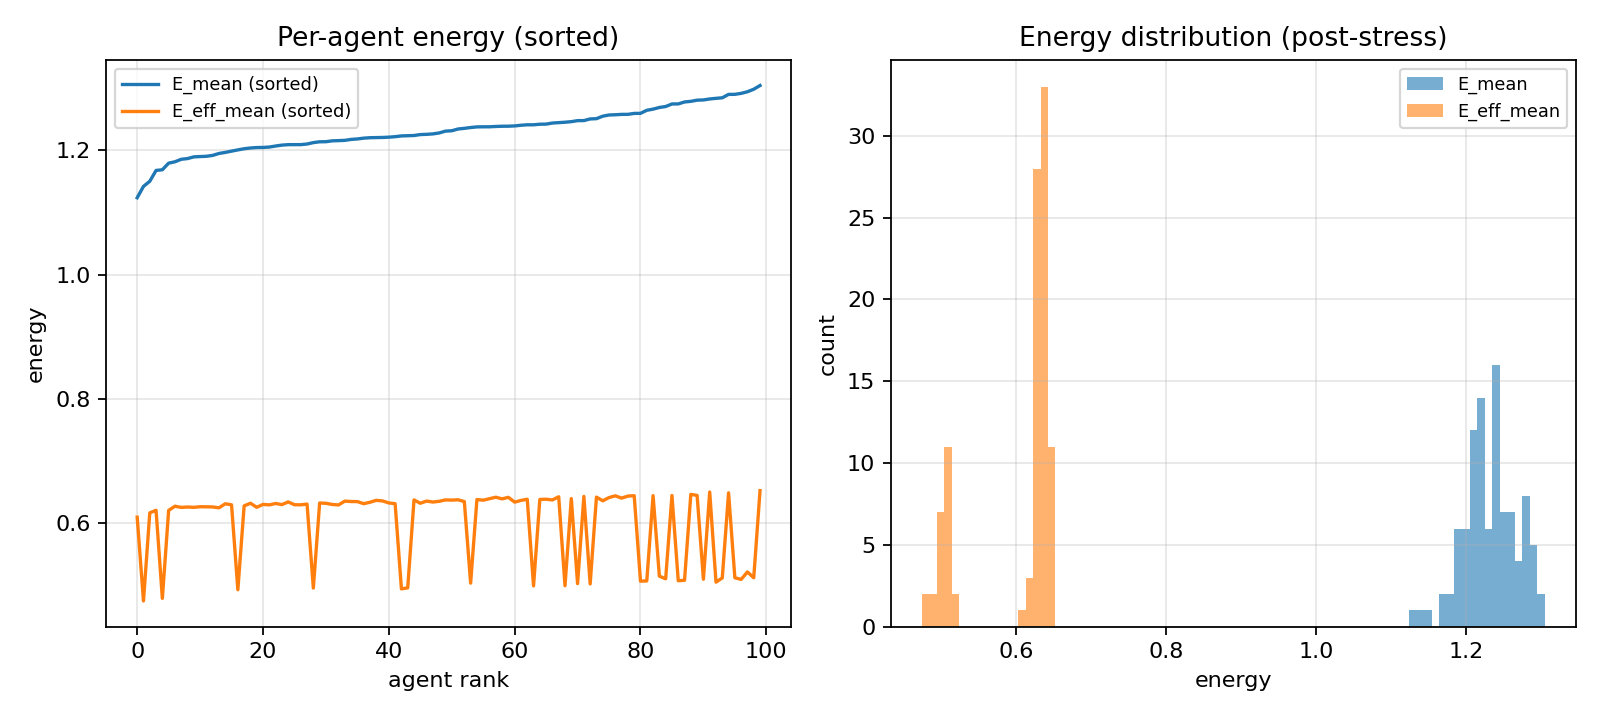
\includegraphics[width=0.9\linewidth]{figures/qrc_per_agent_energy_plot.png}
    \caption{Per-agent energy (sorted and histogram) after stress. $E_{\mathrm{eff}}$ remains lower than $E$ even in the tail.}
    \label{fig:RC_per_agent_energy}
\end{figure}

\paragraph{K saturation under long stress.}
As stress duration grows, the mean $K$ peak rises and then saturates, while recovery time continues to scale with duration.
A first-pass $N=1000$ check shows the same saturation pattern, with $K$ rising to about 69.9 by duration 60 and recovery remaining finite.
This is a single long-stress experiment, not repeated crises: the result supports bounded memory consolidation rather than unbounded accumulation.

\begin{figure}[h]
    \centering
    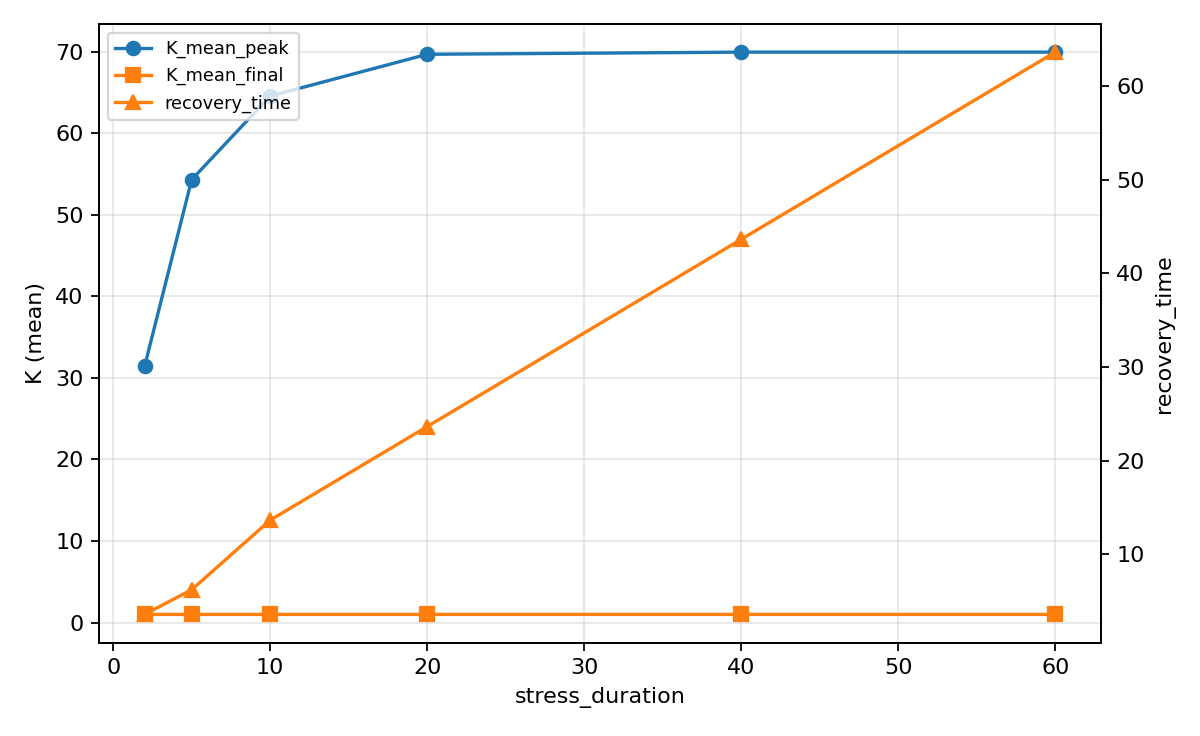
\includegraphics[width=0.9\linewidth]{figures/qrc_k_saturation_plot.png}
    \caption{Mean $K$ peak and recovery time vs stress duration (long-stress regime). $K$ saturates while recovery time continues to grow.}
    \label{fig:RC_k_saturation}
\end{figure}

\paragraph{Critical noise boundary.}
We extend the noise sweep to find the failure threshold. Recovery becomes partial around $\sigma_{noise}\approx 7.7$ and fails beyond $\sigma_{noise}\gtrsim 7.9$ (recovery time becomes NaN).

\begin{figure}[h]
    \centering
    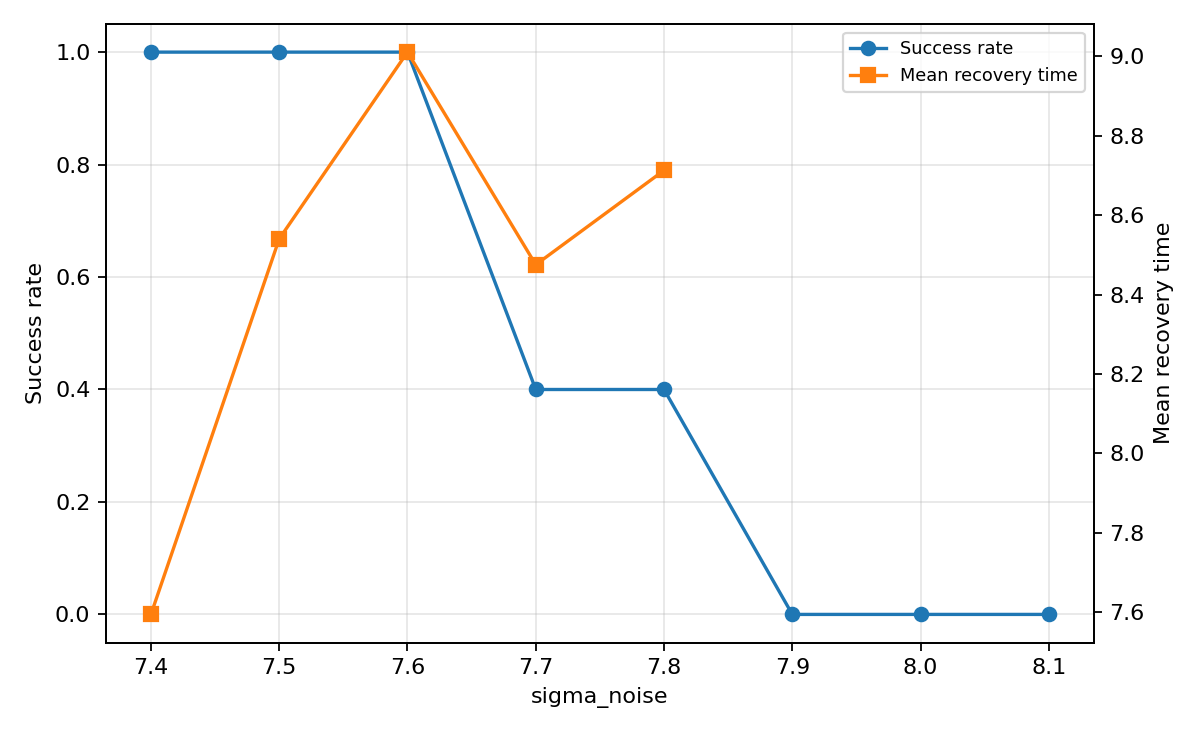
\includegraphics[width=0.9\linewidth]{figures/qrc_noise_boundary_plot.png}
    \caption{Critical noise boundary under RC ($N=100$). Success rate drops sharply between $\sigma_{noise}=7.7$ and $7.9$.}
    \label{fig:RC_noise_boundary}
\end{figure}

\paragraph{Asynchronous delays.}
We test fixed and grouped communication delays. Across the tested delay ranges, recovery remains stable and the success rate stays at 1.

\begin{figure}[h]
    \centering
    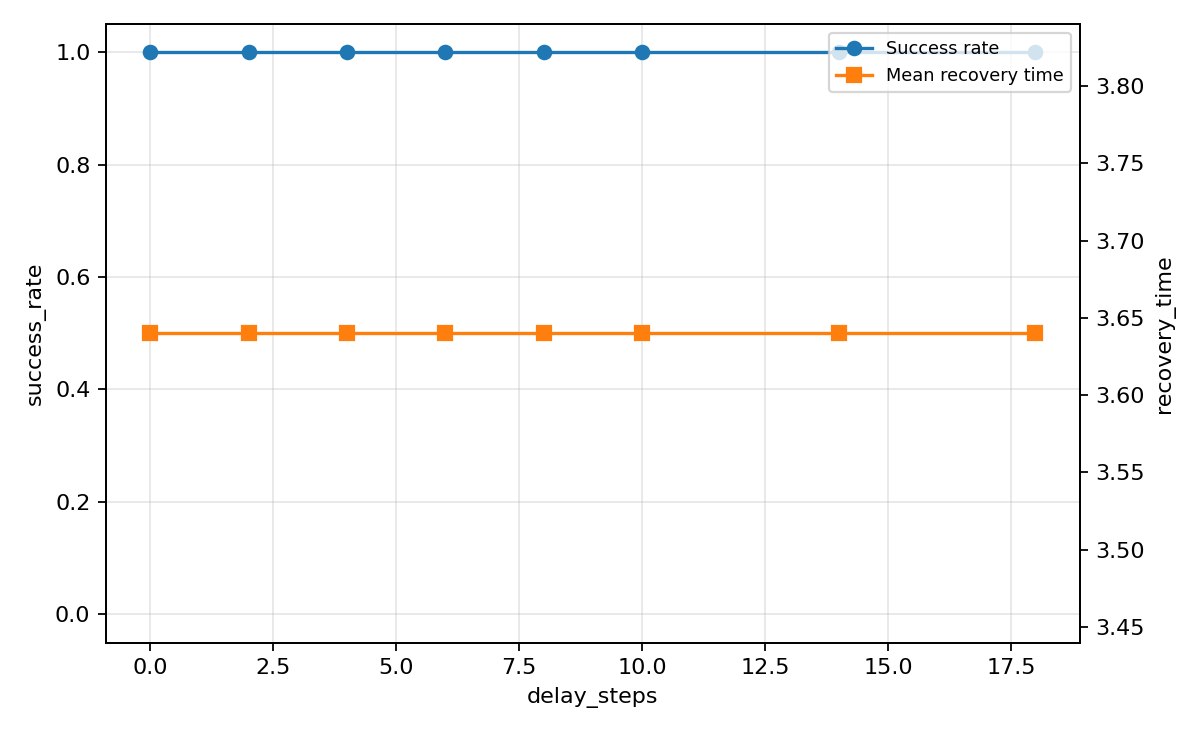
\includegraphics[width=0.9\linewidth]{figures/qrc_delay_boundary_plot.png}
    \caption{Delay robustness (fixed delays). Recovery remains stable across the tested delay steps.}
    \label{fig:RC_delay_boundary}
\end{figure}


\begin{figure}[h]
    \centering
    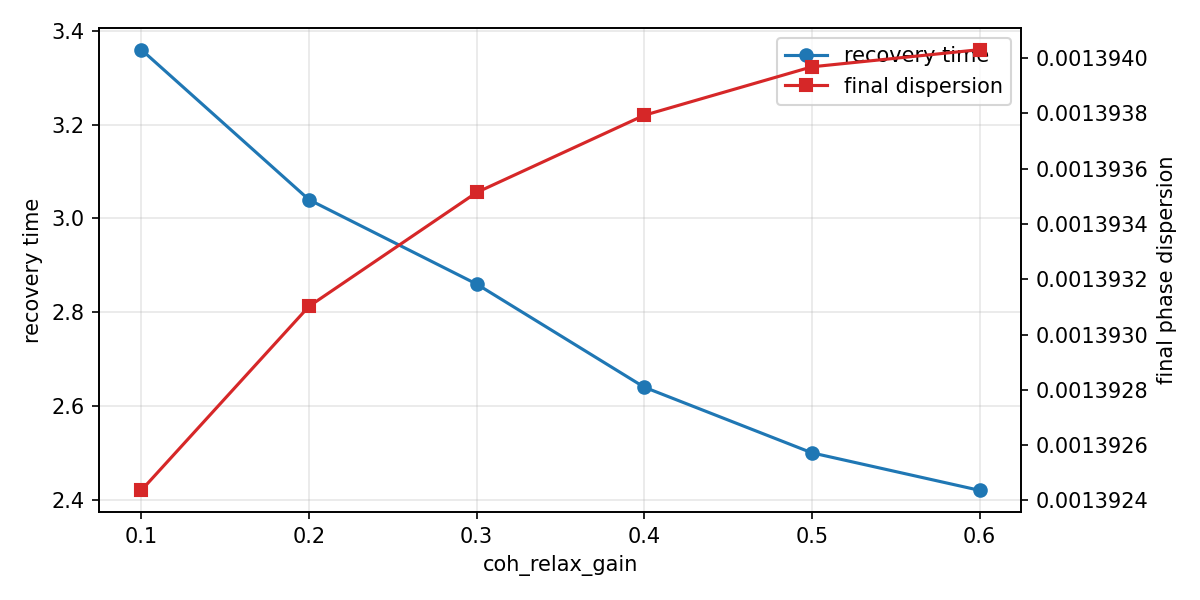
\includegraphics[width=0.9\linewidth]{figures/qrc_cohrelax_sweep_plot.png}
    \caption{Recovery time vs coherence-relax gain $\gamma_{coh}$ (RC on, stress\_frac=0.24).}
    \label{fig:RC_cohrelax}
\end{figure}

\begin{table}[h]
\centering
\small
\begin{tabular}{rrrr}
\toprule
$\gamma_{coh}$ & recovery time & final dispersion & peak mean S \
\midrule
0.1 & 3.36 & 0.0014 & 0.208 \
0.2 & 3.04 & 0.0014 & 0.207 \
0.3 & 2.86 & 0.0014 & 0.206 \
0.4 & 2.64 & 0.0014 & 0.206 \
0.5 & 2.50 & 0.0014 & 0.206 \
0.6 & 2.42 & 0.0014 & 0.205 \
\bottomrule
\end{tabular}
\caption{Sensitivity to coherence-relax gain $\gamma_{coh}$ at fixed stress (RC on).}
\label{tab:RC_cohrelax}
\end{table}

\begin{table}[h]
\centering
\small
\begin{tabular}{lrrrrrrrr}
\toprule
$ f $ & $\tau_{\mathrm{base}}$ & $S_{\max}^{\mathrm{base}}$ & $S_{\infty}^{\mathrm{base}}$ & $\mathcal{D}_{\infty}^{\mathrm{base}}$ & $\tau_{\mathrm{RC}}$ & $S_{\max}^{\mathrm{RC}}$ & $S_{\infty}^{\mathrm{RC}}$ & $\mathcal{D}_{\infty}^{\mathrm{RC}}$ \\
\midrule
0.22 & NaN & 0.2083 & 0.2083 & 0.8744 & 2.42 & 0.2052 & $3.17\times10^{-26}$ & 0.00139 \\
0.24 & NaN & 0.2083 & 0.2083 & 0.8744 & 2.42 & 0.2052 & $3.17\times10^{-26}$ & 0.00139 \\
0.26 & NaN & 0.2500 & 0.2500 & 0.8780 & 3.74 & 0.2463 & $5.87\times10^{-26}$ & 0.00137 \\
\bottomrule
\end{tabular}
\caption{Baseline vs RC outcomes. $\tau$ is recovery time; $S_{\max}$ and $S_{\infty}$ are peak and final mean isolation; $\mathcal{D}_{\infty}$ is final phase dispersion.}
\label{tab:RC_results}
\end{table}

\section{Key Contribution: Coherence-Driven Recovery}
We demonstrate a recovery mechanism that does not rely on hard control or external forcing. In the baseline regime, the network enters an absorbing isolation phase (recovery time diverges). With RC-enabled recognition and coherence-driven relaxation, the system re-enters an active regime with finite recovery time while maintaining high phase coherence. This establishes a concrete, testable mechanism for escaping absorbing phases through informational phase alignment rather than forceful intervention.

\selectlanguage{russian}
\section{Ключевой результат: восстановление на основе когерентности}
Показан механизм восстановления, не требующий жёсткого управления или внешнего принуждения. В базовом режиме сеть переходит в поглощающую фазу изоляции (время восстановления расходится). При включении RC-распознавания и когерентной релаксации система возвращается в активный режим за конечное время и сохраняет высокую фазовую согласованность. Это даёт проверяемый механизм выхода из поглощающих фаз через информационное фазовое согласование, а не через силовое воздействие.
\selectlanguage{english}


\section{Soft Conductor Regime}
We tested a ``soft conductor'' setting with grouped communication delays (60\%/30\%/10\%), small-world topology, and reduced RC gains. The network maintains coherence while allowing local timing diversity.

\selectlanguage{russian}
\section{????? "??????? ????????"}
?? ?????????????? ????? ? ?????????? ?????????? ????? (60\%/30\%/10\%), ?????????? small-world ? ???????????? ?????????????? RC. ???? ????????? ????? ?????????????, ??? ???? ????????? ????????? ???????????? ??????.
\selectlanguage{english}

\begin{figure}[h]
    \centering
    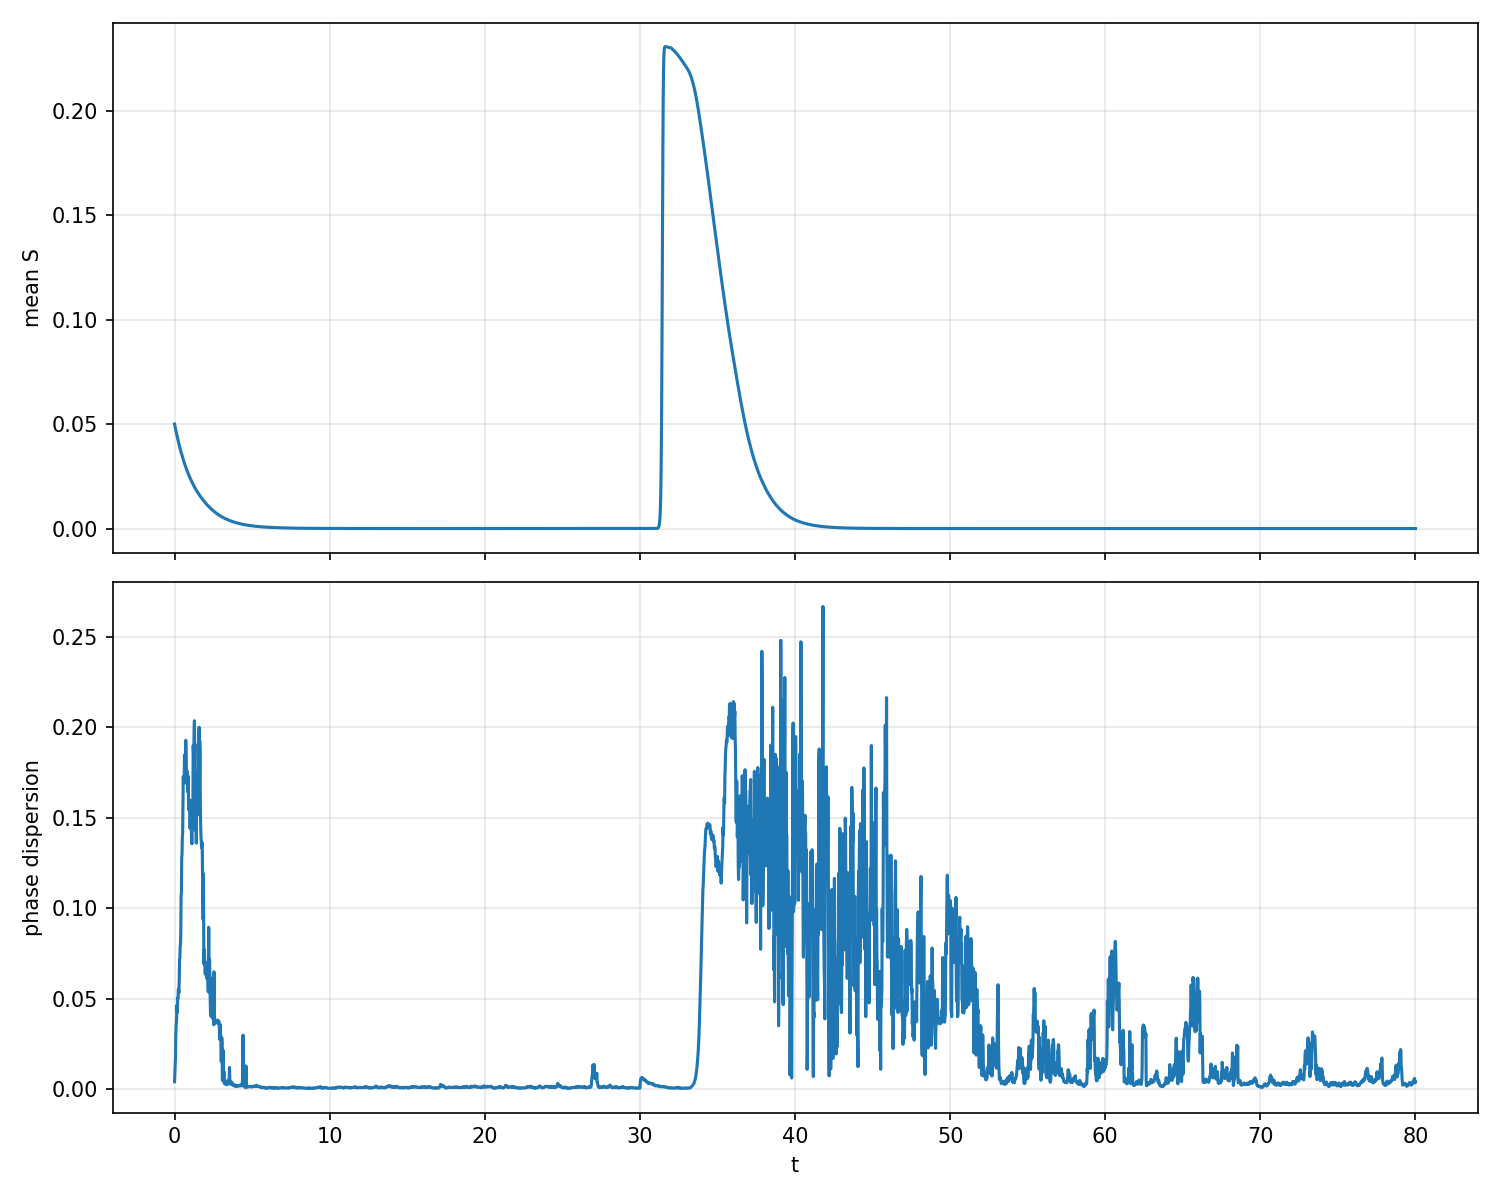
\includegraphics[width=0.9\linewidth]{figures/qrc_soft_conductor_plot.png}
    \caption{Soft conductor regime: grouped delays with small-world topology and reduced RC gains.}
    \label{fig:RC_soft_conductor}
\end{figure}

\section{Experience Accumulation}
We apply repeated stress episodes with fixed amplitude and duration to the same network. Recovery time decreases over episodes, indicating experience accumulation in the adaptive dynamics.

\selectlanguage{russian}
\section{Накопление опыта}
Мы применяем повторяющиеся стресс-эпизоды одинаковой силы и длительности к одной и той же сети. Время восстановления убывает от эпизода к эпизоду, что указывает на накопление опыта в адаптивной динамике.
\selectlanguage{english}

\begin{figure}[h]
    \centering
    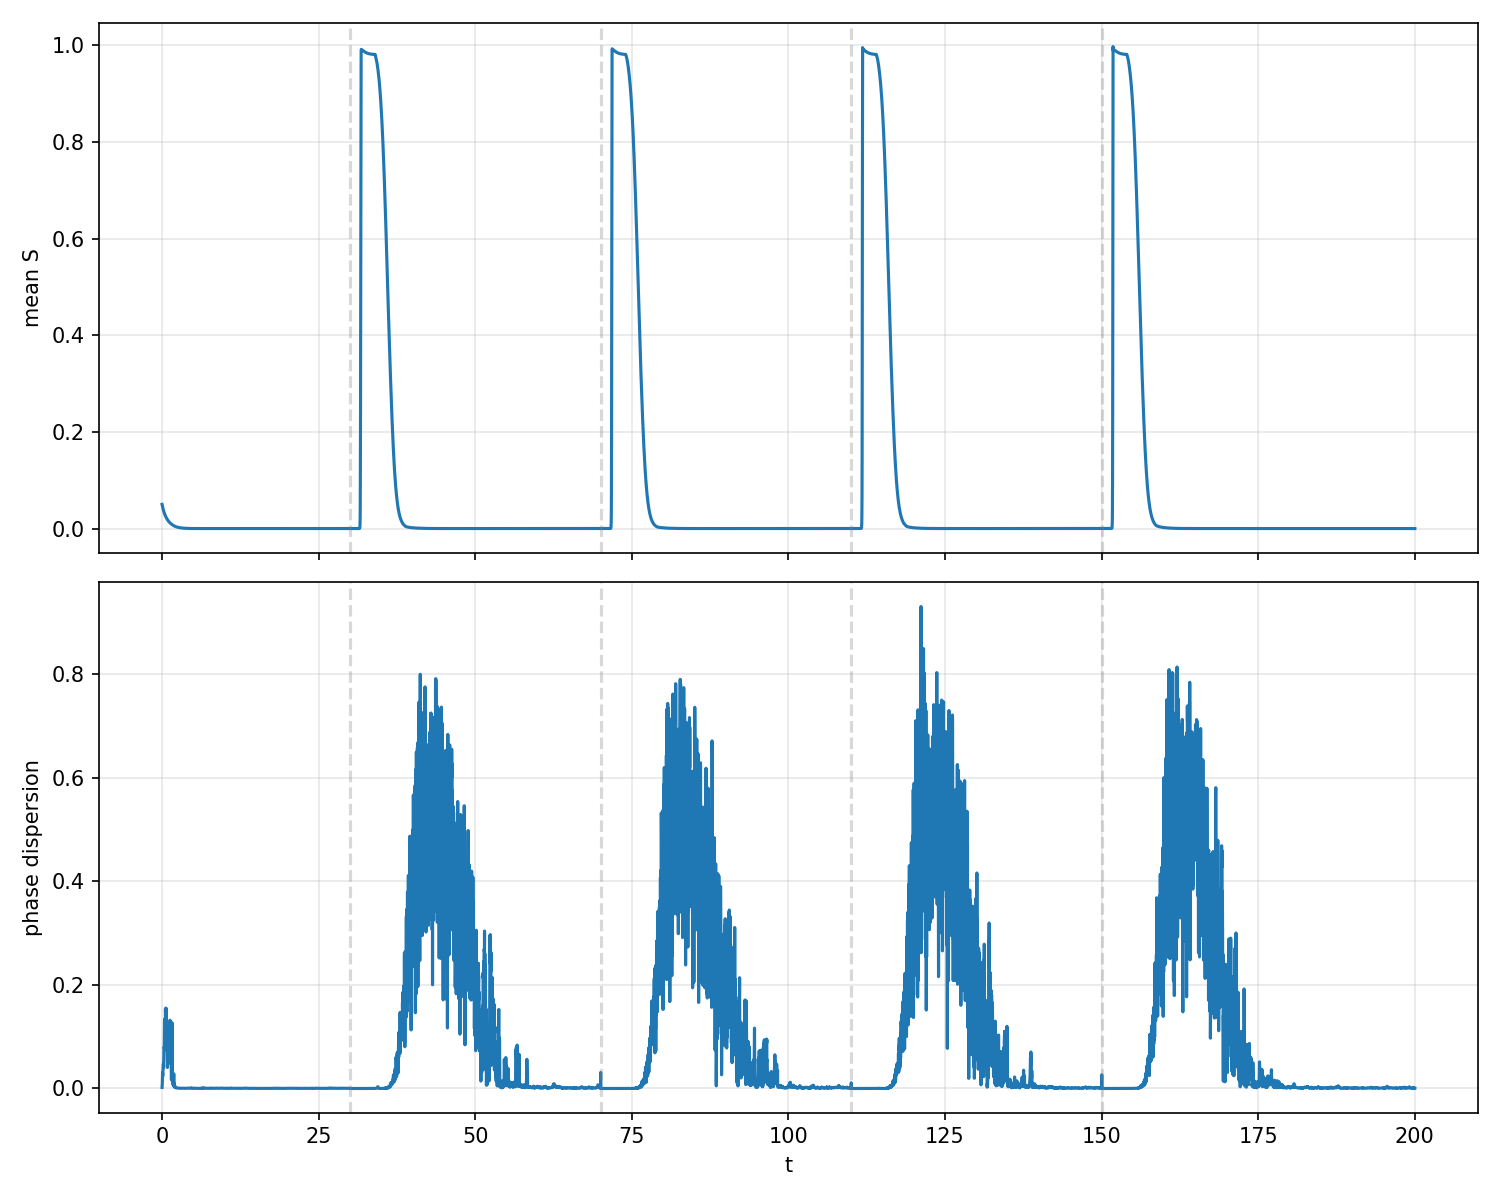
\includegraphics[width=0.9\linewidth]{figures/qrc_multi_stress_plot.png}
    \caption{Repeated stress episodes under RC. Mean isolation recovers faster across episodes.}
    \label{fig:RC_experience}
\end{figure}

\begin{table}[h]
\centering
\small
\begin{tabular}{rrr}
\toprule
episode & stress time & recovery time \\
\midrule
1 & 30 & 126.82 \\
2 & 70 & 86.82 \\
3 & 110 & 46.82 \\
4 & 150 & 6.82 \\
\bottomrule
\end{tabular}
\caption{Recovery time across repeated stress episodes under RC (experience accumulation).}
\label{tab:RC_experience}
\end{table}


\section{Heterogeneous Agents}
We introduced per-agent variability in $\sigma_{noise}$ and $h_{\mathrm{crit}}$ (randomized within 20--30\% bands). The RC mechanism remained effective, yielding finite recovery and low dispersion.

\selectlanguage{russian}
\section{???????????? ??????}
?? ????? ?????????????? ??????? ?????????? $\sigma_{noise}$ ? $h_{\mathrm{crit}}$ (????????? ?????????? ? ???????? 20--30\%). ???????? RC ???????? ?????????????: ?????????????? ????????, ????????? ??????.
\selectlanguage{english}

\paragraph{Per-agent dispersion.}
In a representative heterogeneous run, 76.7\% of agents recovered immediately (per-agent recovery time = 0), 100\% recovered within 6 time units, and about 5\% formed the slow tail near 6. This indicates a small but non-negligible lagging subgroup under heterogeneity.

\selectlanguage{russian}
\paragraph{???????????? ???????.}
? ???????????????? ???????????? ??????? 76.7\% ??????? ?????????????? ????????? (????? ?????????????? = 0), 100\% ?????????????? ?? 6 ?????? ???????, ? ????? 5\% ????????? ????????? ????? ????? 6. ??? ????????? ?? ?????????, ?? ???????? ?????????? ???????????? ???? ??? ??????????????.
\selectlanguage{english}

\begin{figure}[h]
    \centering
    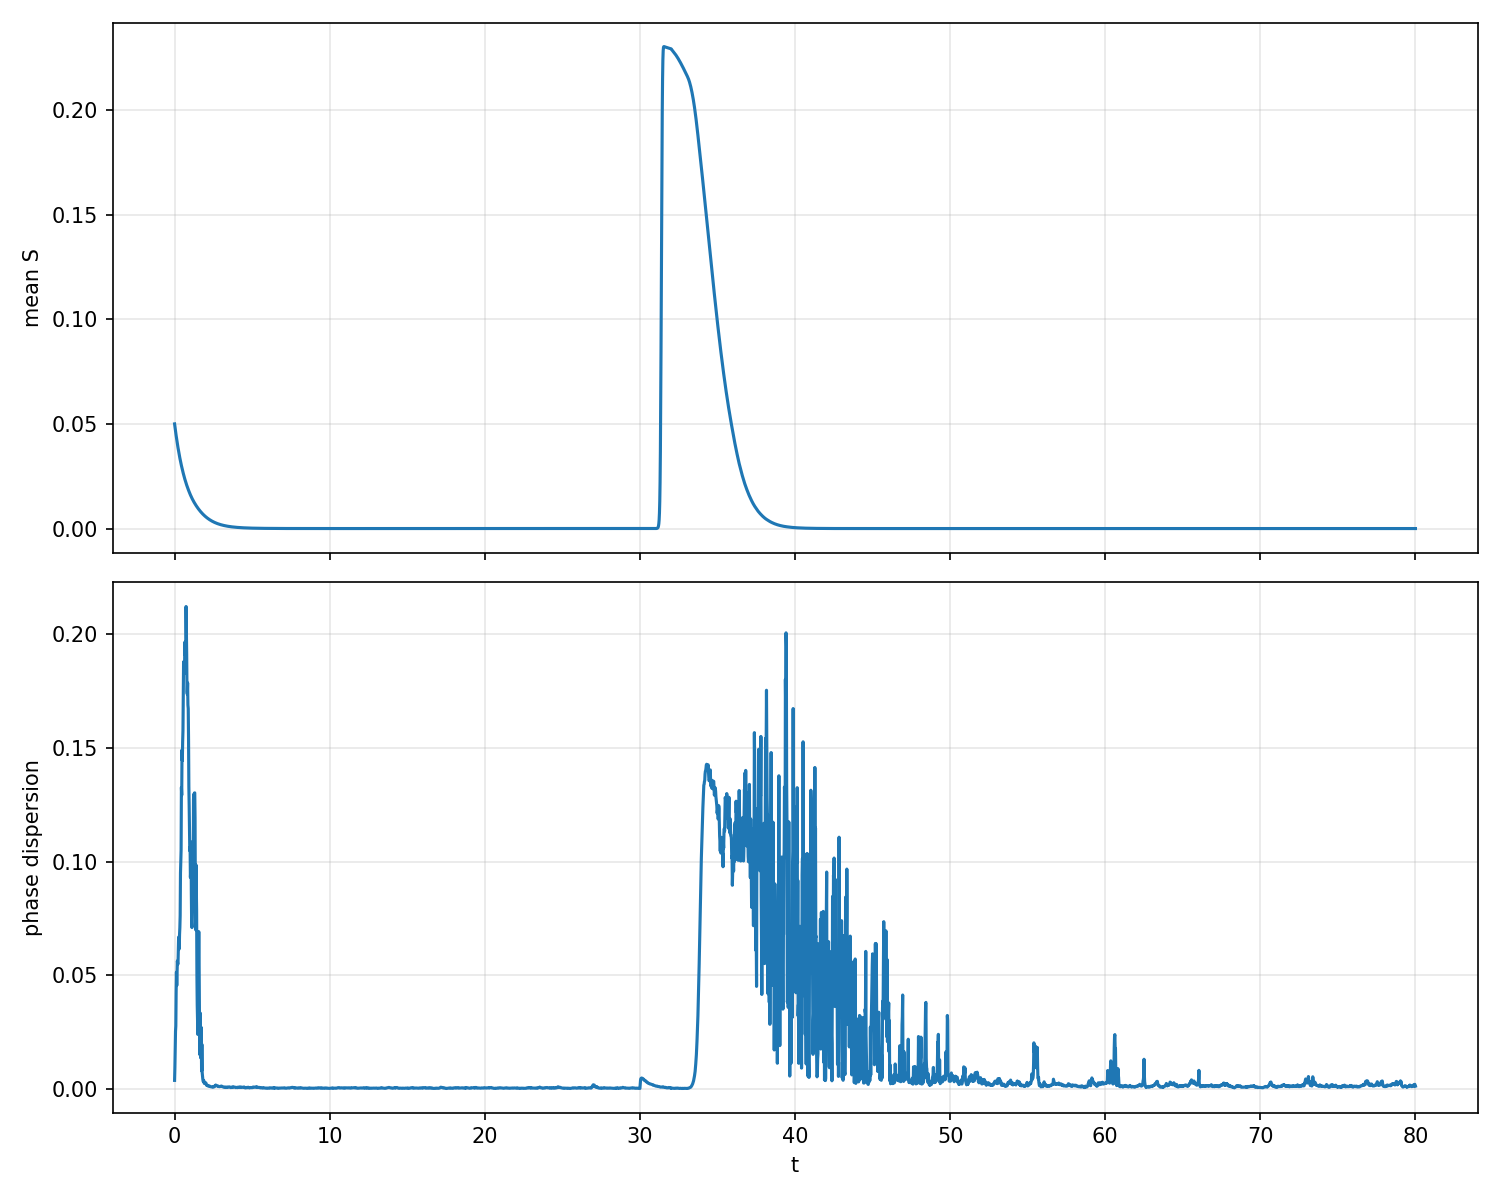
\includegraphics[width=0.9\linewidth]{figures/qrc_heterogeneous_plot.png}
    \caption{Heterogeneous agents (per-agent noise and thresholds) under RC.}
    \label{fig:RC_heterogeneous}
\end{figure}


\section{Heterogeneity Sensitivity (\alpha, \gamma)}
We scanned per-agent variability in $\alpha$ and $\gamma$ (up to ±40\%). Recovery time remained stable and dispersion stayed low, indicating robustness to dynamical heterogeneity.

\selectlanguage{russian}
\section{???????????????? ? ?????????????? (\alpha, \gamma)}
?? ?????????????? ??????? ?????????? $\alpha$ ? $\gamma$ ? ??????? (?? ±40\%). ????? ?????????????? ?????????? ??????????, ? ????????? ??????, ??? ????????? ?? ???????????? ? ???????????? ??????????????.
\selectlanguage{english}

\begin{table}[h]
\centering
\small
\begin{tabular}{rrrr}
\toprule
alpha spread & recovery time & final dispersion & peak mean S \
\midrule
0.1 & 3.56 & 0.0013 & 0.230 \
0.2 & 3.56 & 0.0015 & 0.230 \
0.3 & 3.56 & 0.0017 & 0.230 \
0.4 & 3.56 & 0.0018 & 0.230 \
\bottomrule
\end{tabular}
\caption{Sensitivity to heterogeneity in $\alpha$ (per-agent spread) under RC.}
\label{tab:RC_alpha_spread}
\end{table}

\begin{table}[h]
\centering
\small
\begin{tabular}{rrrr}
\toprule
gamma spread & recovery time & final dispersion & peak mean S \
\midrule
0.1 & 3.56 & 0.0014 & 0.230 \
0.2 & 3.56 & 0.0017 & 0.230 \
0.3 & 3.50 & 0.0011 & 0.230 \
0.4 & 3.52 & 0.0003 & 0.230 \
\bottomrule
\end{tabular}
\caption{Sensitivity to heterogeneity in $\gamma$ (per-agent spread) under RC.}
\label{tab:RC_gamma_spread}
\end{table}


\paragraph{Full heterogeneity summary.}
We compared full heterogeneity at ±20\%, ±30\%, and ±40\% across seeds. Global recovery time remains stable, while the per-agent tail increases with spread.

\selectlanguage{russian}
\paragraph{?????? ?????? ??????????????.}
?? ???????? ?????? ?????????????? ±20\%, ±30\% ? ±40\% ?? ????????????. ?????????? ????? ?????????????? ???????? ??????????, ?? ???????????? "?????" ????????????? ? ?????? ????????.
\selectlanguage{english}

\begin{table}[h]
\centering
\small
\begin{tabular}{rrrrr}
\toprule
spread & recovery time (range) & % immediate & % ≤ 6 & max tail \
\midrule
0.3 & 3.50--3.56 & 73--75 & 97--98 & 12.10 \
0.4 & 3.48--3.62 & 62--65 & 85--92 & 28.26 \
\bottomrule
\end{tabular}
\caption{Full heterogeneity sweep (noise, $h_{crit}$, $\alpha$, $\gamma$). Ranges are across 3 seeds.}
\label{tab:RC_full_hetero}
\end{table}


\section{Energy and Memory (Long Run)}
For a long-run trial ($N=100$, $t_{end}=200$), the recovery time was $pprox 3.66$. Phase dispersion ranged from $1.5	imes10^{-4}$ to $0.15$, while $K_{mean}$ spiked up to $pprox 20.29$ and then relaxed. The effective energy $E_{eff}$ stayed below $E$ throughout.

\selectlanguage{russian}
\section{??????? ? ?????? (??????? ??????)}
? ??????? ??????? ($N=100$, $t_{end}=200$) ????? ?????????????? ????????? $pprox 3.66$. ??????? ????????? ?????? ? ????????? $1.5	imes10^{-4}$--$0.15$, ? $K_{mean}$ ?????????? ?? $pprox 20.29$ ? ????? ??????. ??????????? ??????? $E_{eff}$ ?????????? ???? $E$ ?? ???? ?????????.
\selectlanguage{english}

\section{Applications}
The RC layer provides a formal mechanism for coherence-first recovery in networked systems where hard control is undesirable. Potential applications include:
\begin{itemize}
    \item adaptive multi-agent control with soft synchronization,
    \item hybrid AI systems requiring resilience without hard resets,
    \item coherent architectures where survival depends on phase alignment rather than direct intervention.
\end{itemize}

\selectlanguage{russian}
\section{Применения}
RC обеспечивает формальный механизм восстановления на основе когерентности для сетевых систем, где жёсткое управление нежелательно. Потенциальные применения включают:
\begin{itemize}
    \item адаптивное управление многими агентами с мягкой синхронизацией,
    \item гибридные ��-системы, требующие устойчивости без жёстких сбросов,
    \item когерентные архитектуры, в которых выживание зависит от фазовой согласованности, а не от силовых вмешательств.
\end{itemize}
\selectlanguage{english}

\section{Scope and Limits}
This work does not claim to replace established control or error-correction methods. Its contribution is narrower: it provides a concrete, testable mechanism by which a network can exit an absorbing isolation regime using phase-informational alignment rather than forceful intervention. The novelty is in the combination of (i) isolation-gated coupling, (ii) recognition of coherent phase alignment, and (iii) coherence-driven relaxation of suppression, yielding finite recovery time where the baseline diverges. This is relevant to distributed adaptive systems where hard control is costly, delayed, or undesirable.

\selectlanguage{russian}
\section{Границы применимости}
Мы не заявляем замену классическим методам управления или коррекции ошибок. Вклад этой работы более узкий: показан конкретный, проверяемый механизм выхода сети из поглощающей фазы изоляции через фазово-информационную сонастройку, а не через силовое вмешательство. Новизна в сочетании: (i) изоляционно-гейтированная связь, (ii) распознавание согласованной фазы и (iii) когерентно-управляемая релаксация подавления, что даёт конечное время восстановления там, где базовая динамика расходится. Это релевантно распределённым адаптивным системам, где жёсткий контроль дорог, запаздывает или нежелателен.
\selectlanguage{english}

\section*{Supplementary Appendix: N=1000 (Reserved)}
This appendix is reserved for the larger-scale continuation of the study. It will collect the extended $N=1000$ checks once the longer runs are finalized.
\begin{itemize}
    \item long-run $K$ saturation and tail behavior;
    \item refined critical-noise boundary;
    \item per-agent energy tail at larger scale;
    \item delay sensitivity and grouped-delay robustness.
\end{itemize}
In the first $N=1000$ per-agent energy check, the effective tail cost remained roughly half of the raw tail cost, with $p95$ and $p99$ tail drops near 50\%.
The first $N=1000$ delay check shows stable recovery across the tested fixed and grouped delays, with success rate remaining 1.
The refined $N=1000$ noise sweep places the transition in the $7.9$--$8.3$ corridor, where success drops from 0.6 to 0.2 across the tested seeds.
In the composite boundary run ($\sigma_{noise}=8.0$, grouped delays, and $100$-unit stress duration), RC still recovers but with weakened coherence: recovery time rises to about $112.6$, final dispersion approaches $0.918$, and the effective tail cost remains below the raw tail cost.
The current $K$ result should be read as one long crisis with bounded consolidation. The repeated-episode acceleration remains a separate experiment and will be reported alongside the appendix material.

\selectlanguage{russian}
\section*{Дополнительное приложение: N=1000 (резерв)}
Этот раздел зарезервирован для расширения исследования на более крупный масштаб. Сюда будут собраны завершённые проверки для $N=1000$ после финализации более длинных прогонов.
\begin{itemize}
    \item долгий прогон насыщения $K$ и поведение хвоста;
    \item уточнённая граница критического шума;
    \item хвост пер-агентной энергии на большем масштабе;
    \item чувствительность к задержкам и групповой асинхронности.
\end{itemize}
Текущий результат по $K$ следует читать как один длинный кризис с ограниченной консолидацией опыта. Ускорение восстановления на повторных эпизодах — отдельный эксперимент, который будет вынесен вместе с материалами приложения.
Первая проверка задержек на $N=1000$ показывает устойчивое восстановление в проверенном диапазоне fixed и grouped delays, с успехом 1.
Композитный boundary run ($\sigma_{noise}=8.0$, grouped delays и стресс длительностью $100$) показал, что RC всё ещё восстанавливается, но с ослабленной когерентностью: время восстановления около $112.6$, финальная дисперсия близка к $0.918$, а эффективный хвост энергии остаётся ниже сырого хвоста.
\selectlanguage{english}

\section*{Version Notes (v1)}
\begin{itemize}
    \item Introduced RC as a phase-coordination layer for networked metastable systems.
    \item Added recognition filter and coherence-driven relaxation rule for soft recovery.
    \item Reported baseline vs RC numerical comparison at critical stress fractions.
\end{itemize}

\section*{Acknowledgments}
This work was developed within the conceptual framework of \textbf{Project Symbiosis}, an exploratory research initiative focused on collaborative human--AI theoretical modeling.

The author expresses gratitude to advanced AI systems that contributed to analytical refinement, structural critique, and formulation support during the development of this volume, including:
\begin{itemize}
    \item OpenAI (GPT-series models);
    \item OpenAI Codex (this assistant);
    \item xAI (Grok);
    \item Google DeepMind (Gemini).
\end{itemize}
These systems assisted in iterative mathematical clarification, structural consistency checks, and cross-validation of formal reasoning. All theoretical synthesis, architectural integration, and final responsibility for the presented framework remain with the human author.

\section*{Parameter Summary (Vol I--IV)}
This appendix collects the working parameter values used in simulations and clarifies which thresholds they control.
Key thresholds:
\begin{itemize}
    \item Crisis threshold (Vol II): $C_{\mathrm{crit}} = c_0 e^{-\mu_k K} + \zeta\,\overline{C}$.
    \item Suppression threshold (Vol III): $h_{\mathrm{crit}}$ triggers growth of $S$.
    \item Recognition threshold (Vol IV): $\tau_{recog}$ gates phase-match relaxation.
    \item Coherence gate (Vol IV): $\mathcal{D}=1-|\langle e^{i\theta}\rangle|$; low $\mathcal{D}$ triggers relaxation.
\end{itemize}

\subsection*{Volumes I--II (core / crisis)}
\begin{tabular}{lll}
\toprule
Parameter & Role & Working value \\
\midrule
$\kappa$ & regulator decay ($\Phi$) & 1.2 \\
$\lambda$ & coupling strength & 0.25 \\
$c_0$ & base crisis threshold & 0.45 \\
$\mu_k$ & threshold decay w/ $K$ & 0.25 \\
$\zeta$ & avg crisis weight & 0.55 \\
$\tau$ & crisis window & 6.0 \\
$g_{\min}$ & lower gate bound & 0.15 \\
$\delta_k$ & $K$ decay & 0.3 \\
$\nu$ & $K$ growth from crisis & 0.2 \\
$\xi$ & isolation gain & 0.9 \\
\bottomrule
\end{tabular}

\subsection*{Volume III (memory / stochastic block)}
\begin{tabular}{lll}
\toprule
Parameter & Role & Working value \\
\midrule
$k$ & $x$ decay & 0.8 \\
$\alpha$ & $x\to y$ coupling & 0.9 \\
$\gamma$ & cubic nonlinearity & 0.85 \\
$\sigma_h$ & $y\to H$ gain & 0.35 \\
$\delta_h$ & $H$ decay & 0.45 \\
$\eta_s$ & $S$ suppresses $H$ & 0.55 \\
$\beta$ & $H\to K$ gain & 0.25 \\
$\rho_1,\rho_2,\rho_3$ & $\mu$ dynamics & 0.4, 0.3, 0.35 \\
$\varepsilon_s$ & $S$ speed & 0.6 \\
$h_{\mathrm{crit}}$ & $S$ threshold & 0.7 \\
$\sigma_{noise}$ & noise in $y$ & 0.22 \\
\bottomrule
\end{tabular}

\subsection*{Volume IV (network + QRC)}
\begin{tabular}{lll}
\toprule
Parameter & Role & Working value \\
\midrule
$N$ & agents & 24 (tests at 100) \\
$\Delta t$ & time step & 0.02 \\
$\varepsilon$ & coupling strength & 0.15 \\
$A_{stress}$ & stress amplitude & 1.8 (tests at 3.0) \\
$f$ & stress fraction & 0.22--1.0 \\
$T_{stress}$ & stress duration & 2--20 \\
$\phi_{\mathrm{gain}}$ & QRC pull & 0.5 \\
$\phi_{\mathrm{boost}}$ & QRC boost & 8.0 \\
$g_{\min}^{QRC}$ & QRC lower gate & 0.4 \\
$\tau_{recog}$ & recognition threshold & 0.7 \\
$\gamma_{recog}$ & recognition gain & 1.2 \\
$\gamma_{coh}$ & coherence relax & 0.6 \\
\bottomrule
\end{tabular}

\selectlanguage{russian}
\section*{Сводка параметров (Тома I--IV)}
В этом приложении собраны рабочие значения параметров и указано, какие пороги они задают.
Ключевые пороги:
\begin{itemize}
    \item Порог кризиса (Том II): $C_{\mathrm{crit}} = c_0 e^{-\mu_k K} + \zeta\,\overline{C}$.
    \item Порог подавления (Том III): $h_{\mathrm{crit}}$ включает рост $S$.
    \item Порог распознавания (Том IV): $\tau_{recog}$ включает фазовую релаксацию.
    \item Когерентность (Том IV): $\mathcal{D}=1-|\langle e^{i\theta}\rangle|$; при низкой $\mathcal{D}$ включается релаксация.
\end{itemize}

\subsection*{Тома I--II (ядро / кризис)}
\begin{tabular}{lll}
\toprule
Параметр & Роль & Рабочее значение \\
\midrule
$\kappa$ & затухание регулятора ($\Phi$) & 1.2 \\
$\lambda$ & сила связи & 0.25 \\
$c_0$ & базовый порог кризиса & 0.45 \\
$\mu_k$ & снижение порога с $K$ & 0.25 \\
$\zeta$ & вес среднего кризиса & 0.55 \\
$\tau$ & окно усреднения & 6.0 \\
$g_{\min}$ & нижняя граница гейта & 0.15 \\
$\delta_k$ & распад $K$ & 0.3 \\
$\nu$ & рост $K$ от кризиса & 0.2 \\
$\xi$ & усиление изоляции & 0.9 \\
\bottomrule
\end{tabular}

\subsection*{Том III (память / стохастика)}
\begin{tabular}{lll}
\toprule
Параметр & Роль & Рабочее значение \\
\midrule
$k$ & затухание $x$ & 0.8 \\
$\alpha$ & связь $x\to y$ & 0.9 \\
$\gamma$ & кубическая нелинейность & 0.85 \\
$\sigma_h$ & вклад $y$ в $H$ & 0.35 \\
$\delta_h$ & распад $H$ & 0.45 \\
$\eta_s$ & подавление $H$ через $S$ & 0.55 \\
$\beta$ & вклад $H$ в $K$ & 0.25 \\
$\rho_1,\rho_2,\rho_3$ & динамика $\mu$ & 0.4, 0.3, 0.35 \\
$\varepsilon_s$ & скорость $S$ & 0.6 \\
$h_{\mathrm{crit}}$ & порог $S$ & 0.7 \\
$\sigma_{noise}$ & шум в $y$ & 0.22 \\
\bottomrule
\end{tabular}

\subsection*{Том IV (сеть + QRC)}
\begin{tabular}{lll}
\toprule
Параметр & Роль & Рабочее значение \\
\midrule
$N$ & число агентов & 24 (тесты 100) \\
$\Delta t$ & шаг по времени & 0.02 \\
$\varepsilon$ & сила связи & 0.15 \\
$A_{stress}$ & амплитуда стресса & 1.8 (тесты 3.0) \\
$f$ & доля стресса & 0.22--1.0 \\
$T_{stress}$ & длительность стресса & 2--20 \\
$\phi_{\mathrm{gain}}$ & притяжение к $\Phi$ & 0.5 \\
$\phi_{\mathrm{boost}}$ & усиление QRC & 8.0 \\
$g_{\min}^{QRC}$ & нижняя граница гейта & 0.4 \\
$\tau_{recog}$ & порог распознавания & 0.7 \\
$\gamma_{recog}$ & усиление распознавания & 1.2 \\
$\gamma_{coh}$ & когерентная релаксация & 0.6 \\
\bottomrule
\end{tabular}
\selectlanguage{english}


\section*{DOI}
Project repository: \href{https://github.com/katiasmolskaia-hub/meta-stable-architectures}{https://github.com/katiasmolskaia-hub/meta-stable-architectures}.
Volume IV v1 DOI: to be assigned.

\end{document}


